% !TEX root = ../ac_paper.tex

\section{Stable Andrews--Curtis conjecture and unknot diagrams}\label{sec:stable}

Our focus in this work has so far been on the standard Andrews-Curtis conjecture. In this section, we turn our attention to a closely related variant, known as the “stable” or “weak” Andrews-Curtis conjecture, which is also of great interest, not least because of its connections to algebraic topology. (See e.g. \cite{Meier2016,Bagherifard2021} for recent work on this connection.)
%In \cref{subsec:stable}, we review the statement of this conjecture and present a useful lemma related to it.
%In \cref{subsec:ac-unknot}, we explain a connection between this conjecture and knot theory. 
%Using this connection, new families of potential counterexamples to the standard Andrews-Curtis conjecture were presented in \cite{MMS}. 
%In \cref{sec:proofs}, we will prove that a substantial subclass of these presentations are, in fact, AC-trivial. Furthermore, we conjecture that the remaining presentations are also AC-trivial, supported by evidence from numerous examples.

\subsection{Stable Andrews--Curtis conjecture} \label{subsec:stable}

The stable Andrews--Curtis conjecture, also called the weak Andrews--Curtis conjecture, allows for two further moves in addition to the standard AC-moves (AC1)--(AC3), for the purpose of trivializing a presentation. Namely,
\begin{enumerate}[label=(AC\arabic*)]
	\setcounter{enumi}{3}
	\item Include a new generator and a trivial relator, i.e. replace $\angles{x_1, \dots, x_n \mid r_1, \dots, r_n}$ by $\angles{x_1, \dots, x_n, x_{n+1} \mid r_1, \dots, r_n, x_{n+1}}$.
	\item Remove a trivial relator and the corresponding generator, i.e. the inverse of (AC4).
\end{enumerate}

Two balanced presentations that can be related by a sequence of transformations (AC1)--(AC5) are said to be \textit{stably AC-equivalent}. A presentation that is stably AC-equivalent to a trivial presentation is referred to as \emph{stably AC-trivial}. The stable Andrews-Curtis conjecture states that every balanced presentation is stably AC-trivial. 
%For recent work on connections of this conjecture to algebraic topology, see e.g. \cite{Meier2016,Bagherifard2021}.

As the conjecture allows for addition and removal of new generators and trivial relators, the following lemma is quite useful.

%When simplifying group presentations, it is often useful to decrease the number of generators by substituting an equivalent expression of that generator into all occurrences of it.
%In \cite{BurnsI}, it is mentioned that this move can be executed using (AC1)\UTF{2013}(AC5) when the presentation is of the trivial group.\shehper{@self: I think that MMS is a better reference for this.} We formulate it as a lemma and prove it for self-containment. 

\begin{lemma}[Substitution and Removal]\label{lem:substitution}
    Let $P=\langle x_1,\ldots, x_n, y \mid r_1,\ldots, r_n, y^{-1}w\rangle$ be a presentation of the trivial group, where $w$ is a word in $x_1,\ldots,x_n$. Then $P'=\langle x_1,\ldots, x_n \mid r_1',\ldots, r_n'\rangle$ is stably AC-equivalent to $P$, where $r_i'$ is $r_i$ with all occurrences of $y$ replaced by $w$.
\end{lemma}
\begin{proof}
    First, we substitute $w$ for $y$ in $r_1,\ldots,r_n$, giving $\widetilde{P}=\langle x_1,\ldots,x_n,y\mid r_1',\ldots,r_n',y^{-1}w\rangle$ (cf. \cref{def:ac-sub}). Since $r_1',\ldots,r_n'$ do not contain $y$, we can define the surjective homomorphism $\phi:\widetilde{P}\longrightarrow P'$ by $\phi(x_i)=x_i$ and $\phi(y)=w$. Since $\widetilde{P}$ is trivial, $P'$ is trivial. Therefore, the normal closure of $r_1',\ldots, r_n'$ gives the free group generated by $x_1,\ldots, x_n$, which means $w$ can be written as a product of conjugates of the $r'_i$, namely, $w=w_1 (r_{i_1}')^{\pm1}w_1^{-1}w_2 (r_{i_2}')^{\pm 1}w_2^{-1}\cdots w_m (r_{i_m}')^{\pm 1}w_m^{-1}$, for words $w_i$ in the $x_i$ and $i_k \in \{1,\ldots,n\}$. Note that $m$ may be much larger than $n$. Now using (AC1)--(AC3) we can transform  $y^{-1}w$ to $w_1 (r_{i_1}')^{\pm1}w_1^{-1}\cdots w_m (r_{i_m}')^{\pm 1}w_m^{-1}w^{-1}y$ which equals $y$, and then we can remove $y$ by (AC5).
\end{proof}

%Few steps: 1. use standard substitution to replace $y$ in all of the first $n$ relators. 2. Write a product of conjugates of first $n$ relators that equals $w$. 3. Multiply $y^{-1}w$ with the inverse of this product to get $y^{-1}$.

% TL;DR: the number of AC moves constituting these supermoves is different in the two cases: for vanilla substitution, it is a linear function; but for substitution and removal, we need to supplement vanilla substitution with writing w in terms of other r'_i. The number of AC moves involved in this may be quite large. Specifically, we don't know a bound on m.
We note that, much like the substitution move in the standard Andrews-Curtis conjecture, the \emph{substitution and removal} move can be interpreted as a supermove in the case of stable Andrews-Curtis conjecture. For substitution, the number of AC moves constituting the supermove is a linear function of the lengths of the relators (see \cref{sec:AC}). In contrast, our proof of \cref{lem:substitution} does not yield a similar result for the \emph{substitution and removal} move due to the absence of a bound on $m$. Finding this bound, or discovering an alternative proof of the lemma that establishes such a bound on the number of AC moves packaged into this supermove, would be very useful.

The families of presentations studied in this paper---namely, the Akbulut--Kirby series and the Miller--Schupp series---also serve as potential counterexamples to the stable Andrews--Curtis conjecture.\footnote{Specifically, $\AK(3)$---the shortest potential counterexample for the standard Andrews--Curtis conjecture is also a potential counterexample for the stable Andrews--Curtis conjecture.}
This naturally leads to a broader question about the relationship between the stable Andrews--Curtis conjecture and its standard counterpart: do there exist any stably AC-trivial presentations of the trivial group that could serve as potential counterexamples to the standard Andrews--Curtis conjecture? 
A construction of such candidate presentations from Wirtinger presentations of knot diagrams of the unknot was given in \cite{MMS}. We will review their construction in \cref{subsec:ac-unknot}. In \cref{sec:proofs}, we will prove that a substantial subclass of these presentations are, in fact, AC-trivial. 
% Furthermore, we will conjecture that the remaining presentations are also AC-trivial, supported by evidence from numerous examples.


%One method of finding such presentations is through the knot diagrams of the unknot \cite{MMS}. These presentations are stably AC-trivial by construction, but they could serve as potential counterexamples of the standard Andrews--Curtis conjecture. In \cref{subsec:ac-unknot}, we will review their construction. In \cref{sec:are-all-trivial}, we will prove that a large subclass of these presentations are in fact AC-trivial. We will also provide evidence and hence provide a conjecture that the remaining presentations are also all AC-trivial.

%-----------------------------------------

\subsection{Stably AC-trivial presentations from knot diagrams} \label{subsec:ac-unknot}
%In \cite{MMS}, the authors provided a construction of stably AC-trivial presentations derived from Wirtinger presentations of unknot diagrams. They also used this construction to obtain infinite families of potential counterexamples to the standard Andrews-Curtis conjecture. 
%In this section, we will review their construction.


%In this section, we will review their approach and use it to find new such families. 
%We will also show that a small misprint in their work affects the validity of one of their theorems (\cite[Theorem 1.4]{MMS}). 
%We will also propose a new conjecture for stable AC-trivialization of these presentations and give empirical some evidence in favor of it.

\subsubsection{Stably AC-Trivial Presentations From Wirtinger Presentations}

We recall briefly the construction of the Wirtinger presentations of a knot group. Given any oriented knot diagram with $n$ crossings, we assign generators $\{x_i\}_{i=1}^n$ to each of the arcs, and each crossing gives us a relator $\{r_i\}_{i=1}^n$. In our notation, the left crossing in \cref{fig:wp} corresponds to the relator $y=x^{-1}zx$ and the right one gives $y=xzx^{-1}$. These generators and relators form a balanced presentation of the fundamental group of the knot complement. Moreover, there exists an ordering of the relators and a choice of $\pm 1$ as exponents such that the relators satisfy the equation
$$\prod_{i=1}^nr_i^{\pm1}=1.$$
Thus any relator $r_k$ can be eliminated, giving $\langle x_1,\ldots,x_n\mid r_1,\ldots,r_{k-1},r_{k+1},\ldots,r_n\rangle$, without changing the underlying group. 

\begin{figure}
    \centering
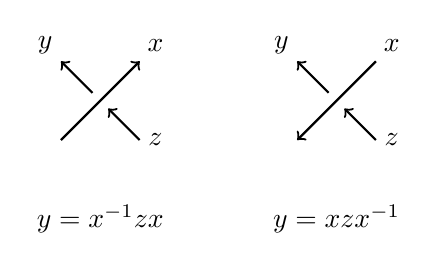
\begin{tikzpicture}
\draw[thick,->] (0,0)--(1,1);
\draw[thick,->] (1,0)--(0.6,0.4);
\draw[thick,->] (0.4,0.6)--(0,1);
\node at (1.2,1.2){$x$};
\node at (-0.2,1.2){$y$};
\node at (1.2,0){$z$};
\node at (0.5,-1){$y=x^{-1}zx$};

\draw[thick,->] (4,1)--(3,0);
\draw[thick,->] (4,0)--(3.6,0.4);
\draw[thick,->] (3.4,0.6)--(3,1);
\node at (4.2,1.2){$x$};
\node at (2.8,1.2){$y$};
\node at (4.2,0){$z$};
\node at (3.5,-1){$y=xzx^{-1}$};

\end{tikzpicture}
    \caption{Types of Crossings}
    \label{fig:wp}
\end{figure}

When the knot is an unknot, the fundamental group of the knot complement is $\mathbb{Z}$, which can be generated by any generator $x_i$. If we add a relator $w$, which is any word in $x_1,\ldots,x_n$ with exponent sum $\pm1$, we get a balanced presentation $\langle x_1,\ldots,x_n\mid r_1,\ldots,r_{k-1},r_{k+1},\ldots,r_n,w\rangle$ of the trivial group. The result below establishes that every such balanced presentation is stably AC-trivial.

\begin{proposition}[Myasnikov, Myasnikov, and Shpilrain, \cite{MMS}] \label{prop:unknot-stable}
    Let $\angles{ x_1,\ldots, x_n\, \mid \, r_1, \ldots, r_n }$ be the Wirtinger presentation of an unknot diagram. Then for any $k=1,\ldots,n$ and word $w$ in the $x_i$ with exponent sum $\pm 1$, the balanced presentation of the trivial group $\langle x_1,\ldots, x_n\,|\, r_1,\ldots, r_{k-1}, r_{k+1},\ldots, r_n, w\rangle$ is stably Andrews-Curtis-trivial.
\end{proposition}

The proof of this proposition relies on the realization of Reidemeister moves for knot diagrams as stable AC moves for the associated balanced presentation of the trivial group. The details of the proof are given in \cref{app:reid}.

\subsubsection{Balanced presentations with fewer generators.}
\label{sec:unknot-gives-potential-counterexamples-ac}
%In \cite{MMS}, the construction above was used as a source of obtaining potential counterexamples of the standard Andrews--Curtis conjecture. However, for the construction to give any interesting presentations, we need a diagram with a large number of crossings. On the other hand, much of the focus in solving potential counterexamples of the Andrews--Curtis conjecture is often placed on presentations with smaller number of generators (as is evidenced by our focus on Akbulut--Kirby and Miller--Schupp families in this paper). 
%A method to reduce the number of generators for any presentation obtained from \cref{prop:unknot-stable} was given in \cite{MMS}, which we review below.
Starting with a balanced presentation coming from \cref{prop:unknot-stable}, one may recursively apply stable AC moves to reduce the number of generators and relators. 
The resultant presentations are all stably AC-trivial by construction, but they could, a priori, serve as potential counterexamples to the standard Andrews--Curtis conjecture \cite{MMS}.\footnote{We will show in the next section, however, that a large subset of these are, in fact, AC-trivial.}

%The resultant presentations, while stably AC-trivial, are potential counterexamples of the standard Andrews-Curtis conjecture \cite{MMS}.

\begin{figure}
    \centering
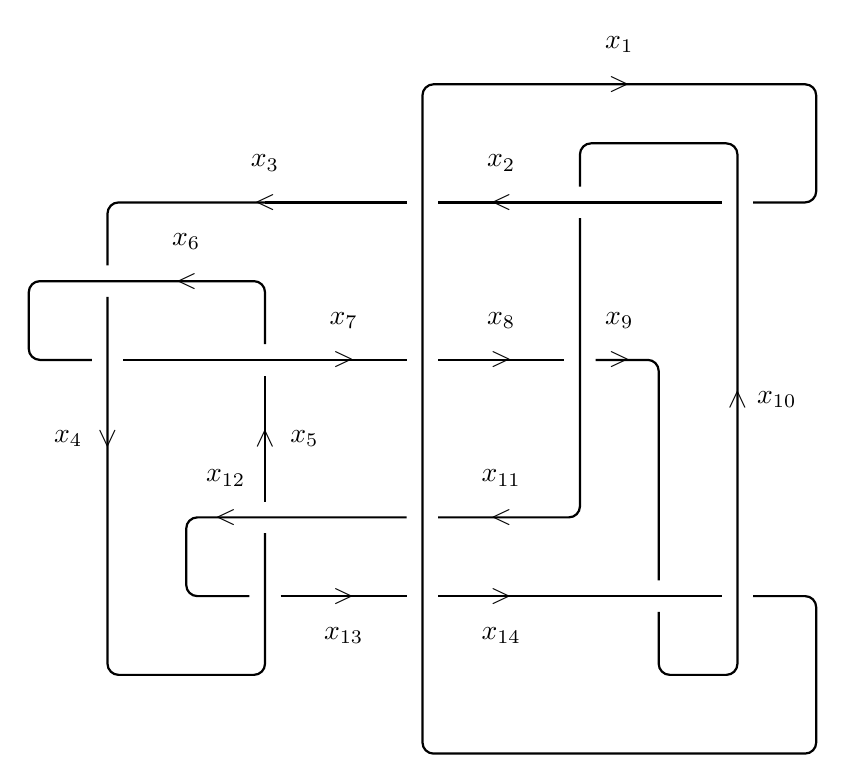
\begin{tikzpicture}
\draw[thick] (0,0)--(1.8,0);
%x3
\draw[thick] (2.2,0)--(5.8,0);
%x2
\draw[thick,rounded corners] (6.2,0)--(7,0)--(7,1.5)--(2,1.5)--(2,-7)--(7,-7)--(7,-5)--(6.2,-5);
%x1
\draw[thick,rounded corners] (0,0)--(-2,0)--(-2,-0.8);
%x3
\draw[thick,rounded corners] (-2,-1.2)--(-2,-6)--(0,-6)--(0,-4.2);
%x4
\draw[thick,rounded corners] (0,-3.8)--(0,-2.2);
%x5
\draw[thick,rounded corners] (0,-1.8)--(0,-1)--(-3,-1)--(-3,-2)--(-2.2,-2);
%x6
\draw[thick,rounded corners] (-1.8,-2)--(1.8,-2);
%x7
\draw[thick,rounded corners] (1.8,-4)--(-1,-4)--(-1,-5)--(-0.2,-5);
%x12
\draw[thick,rounded corners] (0.2,-5)--(1.8,-5);
%x13
\draw[thick,rounded corners] (2.2,-4)--(4,-4)--(4,-0.2);
%x11
\draw[thick,rounded corners] (4,0.2)--(4,0.75)--(6,0.75)--(6,-6)--(5,-6)--(5,-5.2);
%x10
\draw[thick,rounded corners] (2.2,-5)--(5.8,-5);
%x14
\draw[thick,rounded corners] (5,-4.8)--(5,-2)--(4.2,-2);
%x9
\draw[thick,rounded corners] (2.2,-2)--(3.8,-2);
%x8

\node at (4.5,1.5){$>$};
\node at (3,0){$<$};
\node at (0,0){$<$};
\node at (-2,-3){\rotatebox{90}{$<$}};
\node at (0,-3){\rotatebox{90}{$>$}};
\node at (-1,-1){$<$};
\node at (1,-2){$>$};
\node at (3,-2){$>$};
\node at (4.5,-2){$>$};
\node at (6,-2.5){\rotatebox{90}{$>$}};
\node at (3,-4){$<$};
\node at (-0.5,-4){$<$};
\node at (1,-5){$>$};
\node at (3,-5){$>$};

\node at (4.5,2){$x_1$};
\node at (3,0.5){$x_2$};
\node at (0,0.5){$x_3$};
\node at (-2.5,-3){$x_4$};
\node at (0.5,-3){$x_5$};
\node at (-1,-0.5){$x_6$};
\node at (1,-1.5){$x_7$};
\node at (3,-1.5){$x_8$};
\node at (4.5,-1.5){$x_9$};
\node at (6.5,-2.5){$x_{10}$};
\node at (3,-3.5){$x_{11}$};
\node at (-0.5,-3.5){$x_{12}$};
\node at (1,-5.5){$x_{13}$};
\node at (3,-5.5){$x_{14}$};


\end{tikzpicture}
    \caption{Unknot diagram}
    \label{fig:unknot}
\end{figure}


As an example of this procedure, consider the unknot diagram shown in \cref{fig:unknot}. The associated Wirtinger presentation is as follows,
\[
\begin{aligned}
W=\left\langle x_1, x_2, \dots, x_{13}, x_{14} \right. \mid\, &x_1=x_{10} x_{14} x_{10}^{-1}, x_2=x_{10}^{-1} x_1 x_{10},\\
&x_3=x_1^{-1} x_2 x_1, x_4=x_6^{-1} x_3 x_6,\\
&x_5=x_{12} x_4 x_{12}^{-1},x_6=x_7^{-1} x_5 x_7, \\
&x_7=x_4^{-1} x_6 x_4, x_8= x_1 x_7 x_1^{-1}, \\
&x_9=x_{11}^{-1} x_8 x_{11}, x_{10}=x_{14} x_9 x_{14}^{-1} \\
&x_{11}=x_2^{-1} x_{10} x_2, x_{12}=x_1^{-1} x_{11} x_1 \\
& x_{13}=x_4 x_{12} x_4^{-1}, x_{14}=x_1 x_{13} x_1^{-1}\left. \right\rangle .
\end{aligned}
\]

Using stable AC moves, we can reduce the number of generators in $W$ to obtain several 3-generator families of presentations. Consider, for example, deleting the relator $r_6$, adding a word $w$, and eliminating generators in the following order through \cref{lem:substitution}: $x_1$, $x_2$, $x_3$, $x_4$, $x_5$, $x_7$, $x_8$, $x_9$, $x_{11}$, $x_{12}$, and $x_{13}$. We are left with a presentation of three generators $x_6$, $x_{10}$, and $x_{14}$. Renaming $x = x_{10}$, $y = x_{14}$, and $z=x_6$, the resultant presentation equals
\[
\begin{aligned}
\angles{x, y, z \mid & 
% y^{-1} x^{-1} y x 
[y^{-1}, x^{-1}]
y x^{-1} z^{-1} x y^{-1} x^{-1} [y^{-1}, x]
%y^{-1} x y x^{-1} 
z x [y^{-1}, x^{-1}]
% y^{-1} x^{-1} y x
y x^{-1} z x y^{-1} x^{-1}, \\
& % y^{-1} x y x^{-1} 
[y^{-1}, x] z^{-1} x 
%y^{-1} x^{-1} y x 
[y^{-1}, x^{-1}]
y x^{-1} z x y^{-1} 
%x^{-1} y^{-1} x y 
[x^{-1}, y^{-1}]
x y x^{-1} z^{-1} x y^{-1} 
%x^{-1} y^{-1} x y 
[x^{-1}, y^{-1}]
x^{-1} z x y^{-1} x^{-1}, \\
& w}.
\end{aligned}
\]
After choosing an appropriate $w$, we may eliminate one more generator, thus obtaining two-generator presentations through this method. 
%Thus, knot diagrams of the unknot are a useful source of potential counterexamples for the standard Andrews-Curtis conjecture.\lucas{now maybe we contradict this sentence later? at least to some extent}

\begin{remark}
Note, however, that if we were to obtain a 2-generator family without picking a word $w$ (and merely through recursive use of stable AC-moves), we would obtain an infinite family of the form $\angles{ x,y \mid r_1,w }$. Members of this family are all AC-trivial through the following argument. If $\angles{ x,y \mid r_1,w }$ is a presentation coming from an unknot diagram, then $\angles{ x,y \mid r_1 }$ is a presentation of $\mathbb{Z}$ with $r_1 = xy^{\pm 1}$, and any presentation of the form $\angles{ x,y \mid xy^{\pm 1},w }$ is easily AC-trivializable.
\end{remark}

%while this method could give $n$-generator families of potential counterexamples $\angles{x_1, \dots , x_n \mid r_1, \dots, r_{n-1}, w}$ for $n \geq 3$,  any member of a 2-generator family $\angles{ x,y \mid r_1,w }$ thus obtained will be necessarily AC-trivial. This is because if $\angles{ x,y \mid r_1,w }$ is a presentation coming from an unknot diagram, then $\angles{ x,y \mid r_1 }$ must be a presentation of $\mathbb{Z}$. It follows that $r_1 = xy^{\pm 1}$, and any presentation of the form $\angles{ x,y \mid xy^{\pm 1},w }$ is easily AC-trivializable.
%\end{remark}


\begin{remark}
The unknot diagram of \cref{fig:unknot} was originally presented in \cite{MMS}. Their manuscript contained an unfortunate misprint in the 13th relator, where it is written as $x_{13}=x_5 x_{12} x_5^{-1}$.  The resultant presentation is not a Wirtinger presentation of any knot diagram, affecting the validity of one of their main theorems (\cite[Theorem 1.4]{MMS}). For more details, see \cref{app:mms}.
\end{remark}


\subsection{Knot diagrams give AC-trivial presentations} \label{sec:proofs}
In this section, we will prove that every presentation of the form  
 $\angles{ x_1,\ldots, x_n \mid r_1,\ldots, r_{k-1}, r_{k+1},\ldots, r_n, w}$ as in \cref{prop:unknot-stable}, is in fact AC-trivial. Moreover, we will show that presentations with fewer generators that come from recursively applying \cref{lem:substitution} are also AC-trivial. 
% Finally, we will propose that all presentations with fewer generators also all AC-trivial and therefore do not provide potential counterexamples to the standard Andrews--Curtis conjecture.

The proofs of AC-triviality rely on the following lemma, which establishes that presentations with different choices of $w$ are all AC-equivalent. 

\begin{lemma}
\label{lem:all_ac_equiv}
    Let $\langle x_1,\ldots, x_n \mid r_1,\ldots,r_{n-1}\rangle$ be a presentation of $\mathbb{Z}$. Then there exists one word $x$ in the $x_i$, such that for any word $w$ that makes the group trivial, the balanced presentation of the trivial group $\langle x_1,\ldots, x_n \mid r_1,\ldots,r_{n-1}, w\rangle$ is AC-equivalent to $\langle x_1,\ldots, x_n \mid r_1,\ldots,r_{n-1}, x\rangle$.
\end{lemma}

\begin{proof}[Proof]
    Since $\langle x_1,\ldots, x_n \mid r_1,\ldots,r_{n-1}\rangle$ is a presentation of $\mathbb{Z}$, there exists one word $x$ that generates $\mathbb{Z}$. Then any $x_i$ can be given by the product of $x^{n_i}$ with a product of conjugates of $r_1,...,r_{n-1}$ for some $n_i\in\mathbb{Z}$.

Suppose $w=x_{i_1}^{\epsilon_ 1}x_{i_2}^{\epsilon_2}\cdots x_{i_m}^{\epsilon_m}$ for $i_k\in \{1,\ldots,n\}$ and $\epsilon_k\in\mathbb{Z}$. For each $x_i$ in $w$, multiply $w$ by the corresponding product of conjugates of $r_1,...,r_{n-1}$ to replace $x_i$ by $x^{n_i}$. Then $w$ is changed to $x^p$ for some $p$. Since $x$ generates $\mathbb{Z}$, $p=\pm 1$. 
\end{proof}

Note that the lemma holds for \emph{any} presentation $\langle x_1,\ldots, x_n \mid r_1,\ldots,r_{n-1}\rangle$ of $\mathbb{Z}$, and not just the ones coming from knot diagrams of the unknot. We will now use this lemma to prove our result for presentations of \cref{prop:unknot-stable}.

\begin{theorem} \label{prop:unknot}
    Let $\angles{ x_1,\ldots, x_n\, \mid \, r_1, \ldots, r_n }$ be the Wirtinger presentation of an unknot diagram. Then for any $k=1,\ldots,n$ and word $w$ in the $x_i$ with exponent sum $\pm 1$, the balanced presentation of the trivial group $\angles{ x_1,\ldots, x_n \mid r_1,\ldots, r_{k-1}, r_{k+1},\ldots, r_n, w}$ is Andrews--Curtis-trivial.
\end{theorem}

\begin{proof}
The relation  $$\prod\limits_{i=1}^nr_i^{\pm1}=1$$ for a Wirtinger presentation of a knot diagram allows us to write any one relator $r_i$ as a product of other relators and their inverses. Hence, the presentations 
$$\angles{x_1, \ldots, x_n \mid r_1, \ldots, r_{k-1}, r_{k+1}, \ldots, r_n, w}$$ with different choices of $k \in \{1, \ldots, n\}$ and fixed $w$ are all AC-equivalent. Without loss of generality, we set $k=n$. As the presentation comes from a Wirtinger presentation, we can write it as 
\[
\angles{ x_1,\ldots,x_n \mid x_1=z_2x_2z_2^{-1}, x_2=z_3x_3z_3^{-1},\ldots, x_{n-1}=z_{n}x_nz_{n}^{-1}, w },
\]
where $z_i\in \{x_1^{\pm 1},\ldots, x_n^{\pm 1}\}$. 

Using \cref{lem:all_ac_equiv}, we choose $w = x_n$. 
With the second-last relator \( x_{n-1} = z_{n-1} x_n z_{n-1}^{-1} \), substituting \( x_n = 1 \) simplifies it to \( x_{n-1} = 1 \). Substituting \( x_{n-1} = 1 \) into the preceding relator, we proceed iteratively, simplifying each relation until the first relation reads \( x_1 = 1 \). 
Thus, the presentation reduces to  $\angles{x_1, \ldots, x_n \mid x_1, \ldots, x_n}$,
rendering it AC-trivial. 
% As the last relator is $x_{n-1}=z_{n-1}x_nz_{n-1}^{-1}$, we can substitute $x_n=1$ into the relator, simplifying it to $x_{n-1}$. We then substitute $x_{n-1}=1$ into the previous relator, and continue this process until the first relator reads $x_1$. We get the presentation $\langle x_1,\ldots, x_n\,|\, x_1,\ldots,x_n\rangle$, rendering the presentation in question AC-trivial. 
\end{proof}
\begin{remark}
    Starting with a balanced presentation of \cref{prop:unknot} and reducing the number of generators only through recursive application of substitution and removal (\cref{lem:substitution}), we obtain a large class of AC-trivial presentations with fewer generators. Indeed, each relator in any such presentation is still a simple conjugation relation ($x_i=zx_jz^{-1}$ where $z$ is some word in the generators). Thus we can use the same argument as in the proof of \cref{prop:unknot} to trivialize the relators iteratively. 
\end{remark}

For example, consider the 3-generator family presented in the previous section, which was obtained through repeated application of \cref{lem:substitution}. The first relator is $x$ equals $z$ conjugated by  $yxyx^{-1}z^{-1}xy^{-1}x^{-1}y^{-1}xyx^{-1}$, and the second relator is $y$ equals $x$ conjugated by $xyx^{-1}z^{-1}xy^{-1}x^{-1}yxyx^{-1}zxy^{-1}x^{-1}y^{-1}$. Substituting $w=z$ simplifies the first relator to $x$, which when substituted into the second relator, simplifies it to $y$. 
% \lucas{I don't think this conjecture really makes sense anymore: we know that presentations coming from knot diagram directly are AC-trivial. Thus, to conjuecture that we can do any stable AC move and get something still AC trivial is just to conjecture that the stable AC conjecture isn't actually any weaker than the AC conjecture. \fixme{Shehper: Not really. We are making this claim not in general but only for presentations coming from knot diagrams. So perhaps, yes, if you'd like, the conjecture is that for presentations coming from knot diagrams, all being stably AC-trivial, are also AC-trivial.

% I am okay with whether you'd want to include this conjecture or not. We'll just need to edit the last two sentences of Section 8.1 where we say "In subsection 8.3..." and also the introduction of the paper where we also mention the conjecture accordingly.}}
% We used this procedure for a large class of presentations with fewer generators, derived from various knot diagrams of the unknot, including several ``hard" diagrams presented in \cite{burton2024hard}. We found that in each case, there existed a simple choice of $w$ that trivialized the presentation. Therefore, we hypothesize that knot diagrams only give AC-trivial presentations. Establishing a general proof of this statement would be a significant contribution and is left as an open question for future research.


% \subsection{New work}
% \shehper{@self: based on Lucas' conjecture, new rewriting of section 8 could be as follows.

% At the moment, the way I understand things is that we have shown AC-triviality of balanced presentations coming from Unknot diagrams. So section 8.2.1 should be expanded and perhaps turned into a section of its own. Section 8.2.2 would become section 8.3 with the example. 

% Alternatively, if Lucas' conjecture says that the 3-generator presentation studied in 8.2.2 is also AC-trivial, then we will probably want to rewrite in a different way.. The main hero of the story then is proposition 14. We will either rewrite conjecture 15 to include all lower-generator presentations as well, or we will include a conjecture 16 that is about lower-generator presentations. We can include conjecture 15 in Section 8.2.1. Section 8.2.2 will be the example of W along with derivation of its AC-triviality. 
% }
% Moreover, we note that all such presentations are all AC-equivalent. Using the fact that 
% \[\langle x_1,\ldots, x_n\,|\, r_1,\ldots, r_{k-1}, r_{k+1},\ldots, r_n, w\rangle\] and \[\langle x_1,\ldots, x_n\,|\, r_1,\ldots, r_{\ell-1}, r_{\ell+1},\ldots, r_n, w\rangle\] for any $k,\ell\in \{1,\ldots, n\}$
% are AC-equivalent, this follows as a corollary of the following proposition:

% %--- old, specific version
% %\begin{proposition}
% %    Let $\angles{ x_1,\ldots, x_n\, \mid \, r_1, \ldots, r_n }$ be the Wirtinger presentation of an unknot diagram. Then for any $k=1,\ldots,n$ and word $w$ in the $x_i$ with exponent sum $\pm 1$, the balanced presentation of the trivial group $\langle x_1,\ldots, x_n\,|\, r_1,\ldots, r_{k-1}, r_{k+1},\ldots, r_n, w\rangle$ is  Andrews-Curtis equivalent to $\langle x_1,\ldots, x_n\,|\, r_1,\ldots, r_{k-1}, r_{k+1},\ldots, r_n, x_1\rangle$, i.e., the presentation from choosing $w=x_1$.
% %\end{proposition}
% %\begin{proof}
%  %   The presentation $\langle x_1,\ldots, x_n\,|\, r_1,\ldots, r_{k-1}, r_{k+1},\ldots, r_n \rangle$ is a presentation of $\mathbb{Z}$, so the normal closure of $r_1,\ldots, r_{k-1}, r_{k+1},\ldots, r_n$ is $\langle x_1=x_2,\ldots,x_1=x_{k-1},x_1=x_{k+1},\ldots, x_1=x_n\rangle$. Thus, if the last element of $w$ is $x_i$, we can construct $x_i^{-1}x_1$ as a product of conjugates of the relators $r_1,\ldots, r_{k-1}, r_{k+1},\ldots, r_n$. We then conjugate by $x_1$ and repeat this process until every element of $w$ has been converted into $x_1$. Since the exponent sum of $w$ is $\pm 1$, this can be simplified to just $x_1^{\pm 1}$. We can invert the relation if necessary so that it simply reads $x_1$. 
% %\end{proof}
% %\begin{proposition}
% %\label{prop:all_ac_equiv}
% %    Let $\langle x_1,\ldots, x_n \mid r_1,\ldots,r_{n-1}\rangle$ be a presentation of $\mathbb{Z}$. Then for any word $w$ in the $x_i$ with exponent sum $\pm 1$, the balanced presentation of the trivial group $\langle x_1,\ldots, x_n \mid r_1,\ldots,r_{n-1}, w\rangle$ is AC-equivalent to $\langle x_1,\ldots, x_n \mid r_1,\ldots,r_{n-1}, x_1\rangle$.
% %\end{proposition}
% %\begin{proof}
% %    Let $w=x_{i_1}^{\epsilon_ 1}x_{i_2}^{\epsilon_2}\cdots x_{i_m}^{\epsilon_m}$ for $i_k\in \{1,\ldots,n\}$ and $\epsilon_k\in \{-1,1\}$, where we assume without loss of generality that $\epsilon_m=1$. By assumption, $\sum_{k=1}^m \epsilon_k=\pm 1$. 
    
% %    Since $\langle x_1,\ldots, x_n \mid r_1,\ldots,r_{n-1}\rangle$ is a presentation of $\mathbb{Z}$, the normal closure of $r_1,\ldots, r_{n-1}$ is $\langle x_1x_2^{-1},x_1x_3^{-1},\ldots, x_1x_{n-1}^{-1}\rangle$. This means we can express $w'=x_{i_m}^{-1}x_1$ as product of conjugates of $r_1,\ldots,r_{n-1}$. Multiplying $w$ by $w'$ gives $x_{i_1}^{\epsilon_ 1}x_{i_2}^{\epsilon_2}\cdots x_{i_{m-1}}^{\epsilon_{m-1}}x_1$. Now we conjugate by $x_1$ and repeat this process. As the exponent sum of $w$ is $\pm 1$, this will eventually simplify $w$ into $x_1^{\pm 1}$. Inverting if necessary gives the result. 
% %\end{proof}

% \begin{proposition}
% \label{prop:all_ac_equiv}
%     Let $\langle x_1,\ldots, x_n \mid r_1,\ldots,r_{n-1}\rangle$ be a presentation of $\mathbb{Z}$. Then there exists one word $x$ in the $x_i$, such that for any word $w$ that makes the group trivial, the balanced presentation of the trivial group $\langle x_1,\ldots, x_n \mid r_1,\ldots,r_{n-1}, w\rangle$ is AC-equivalent to $\langle x_1,\ldots, x_n \mid r_1,\ldots,r_{n-1}, x\rangle$.
% \end{proposition}
% \begin{proof}
%     Since $\langle x_1,\ldots, x_n \mid r_1,\ldots,r_{n-1}\rangle$ is $\mathbb{Z}$, there exists one word $x$ that generates $\mathbb{Z}$. Then any $x_i$ can be given by the product of $x^{n_i}$ with a product of conjugates of $r_1,...,r_{n-1}$ for some $n_i\in\mathbb{Z}$.

%     Suppose $w=x_{i_1}^{\epsilon_ 1}x_{i_2}^{\epsilon_2}\cdots x_{i_m}^{\epsilon_m}$ for $i_k\in \{1,\ldots,n\}$ and $\epsilon_k\in\mathbb{Z}$. For each $x_i$ in $w$, multiply $w$ by the corresponding product of conjugates of $r_1,...,r_{n-1}$ to replace $x_i$ by $x^{n_i}$. Then $w$ is changed to $x^p$ for some $p$. Since $x$ generates $\mathbb{Z}$, $p=\pm 1$. 
% \end{proof}


% In \cref{sec:unknot-gives-potential-counterexamples-ac}, we discuss how unknots give potential counterexamples to the Andrews-Curtis conjecture. However, we find that the presentations from which these counterexamples come are AC-trivial. 
% \begin{proposition}
%     Exact same statement as \cref{prop:unknot}
%  just remove stable:    Any presentation \[\langle x_1,\ldots, x_n\,|\, r_1,\ldots, r_{k-1}, r_{k+1},\ldots, r_n, w\rangle\] coming from an unknot as in \cref{prop:unknot} is AC-trivial.
% \end{proposition}
% \begin{proof}
% Without loss of generality, we let $k=n$.\lucas{depending on how we mention whats at the beginning of this section I should maybe specify why this is allowed} Then since the presentation $\langle x_1,\ldots, x_n\,|\, r_1,\ldots,r_{n-1}\rangle$ comes from a Wirtinger presentation, we can write it as 
% \[
% \langle x_1,\ldots,x_n \mid x_1=z_2x_2z_2^{-1}, x_2=z_3x_3z_3^{-1},\ldots, x_{n-1}=z_{n}x_nz_{n}^{-1}\rangle,
% \]
% where $z_i\in \{x_1^{\pm 1},\ldots, x_n^{\pm 1}\}$.

% % need to do more work here

% Now we choose $w$ to be $x_n$. Since the last relator is $x_{n-1}=z_{n-1}x_nz_{n-1}^{-1}$, we can substitute $x_n=1$ into the relator, and it simplifies into $x_{n-1}$. We then substitute $x_{n-1}=1$ into the previous relator, and continue this process until the first relator reads $x_1$. We get the presentation $\langle x_1,\ldots, x_n\,|\, x_1,\ldots,x_n\rangle$, and thus it is AC-trivial. 

% \end{proof}

% ALL UNNCESSARY NOW
% ----------------------
% By \cref{prop:all_ac_equiv}, for a fixed unknot, all such presentations are AC-equivalent, so it suffices to show it for a single choice of $k$ and $w$. 

% Consider by means of example the unknot in \cref{fig:unknot}. The Wirtinger presentation of the knot is 
% \[
% \begin{aligned}
% \left\langle x_1, x_2, x_3, x_4, x_5, x_6, x_7, x_8, x_9, x_{10}, x_{11}, x_{12}, x_{13}, x_{14} \right. \mid\, &x_1=x_{10} x_{14} x_{10}^{-1}, x_2=x_{10}^{-1} x_1 x_{10},\\
% &x_3=x_1^{-1} x_2 x_1, x_4=x_6^{-1} x_3 x_6,\\
% &x_5=x_{12} x_4 x_{12}^{-1},x_6=x_7^{-1} x_5 x_7, \\
% &x_7=x_4^{-1} x_6 x_4, x_8= x_1 x_7 x_1^{-1}, \\
% &x_9=x_{11}^{-1} x_8 x_{11}, x_{10}=x_{14} x_9 x_{14}^{-1} \\
% &x_{11}=x_2^{-1} x_{10} x_2, x_{12}=x_1^{-1} x_{11} x_1 \\
% & x_{13}=x_4 x_{12} x_4^{-1}, x_{14}=x_1 x_{13} x_1^{-1}\left. \right\rangle
% \end{aligned}
% \]

% We remove the last relation $x_{14}=x_1x_{13}x_1^{-1}$ and fix $w=x_1$. We start by substituting $x_1=x_{10}x_{14}x_{10}^{-1}$ into the second relation, which gives $x_2=x_{14}$. This allows us to replace all other instances of $x_{14}$ with $x_2$. In particular, the tenth relation now reads $x_{10}=x_2 x_9 x_{2}^{-1}$ which we substitute into the eleventh relation to get $x_9=x_{11}$.  We then replace all other instances of $x_{11}$ with $x_9$, which turns the ninth relation into $x_9=x_8$. We replace all other instances of $x_9$ with $x_8$. 

% Our relations now read
% \[
% \begin{aligned}
% &x_1=x_{10} x_{2} x_{10}^{-1}, x_2=x_{14}, x_3=x_1^{-1} x_2 x_1, x_4=x_6^{-1} x_3 x_6, x_5=x_{12} x_4 x_{12}^{-1},\\
% &x_6=x_7^{-1} x_5 x_7, x_7=x_4^{-1} x_6 x_4, x_8= x_1 x_7 x_1^{-1}, x_9= x_8, x_{10}=x_{2} x_8 x_{2}^{-1} \\
% &x_{11}=x_9, x_{12}=x_1^{-1} x_{8} x_1, x_{13}=x_4 x_{12} x_4^{-1},x_1.
% \end{aligned}
% \]

% We now substitute $x_8= x_1 x_7 x_1^{-1}$ into the twelfth relation, which gives $x_{12}=x_7$, and we replace all other occurrences of $x_{12}$ with $x_7$. The fifth relation now reads $x_5=x_7 x_4 x_7^{-1}$. We substitute this into the sixth relation, which gives $x_6=x_4$, and we replace every other occurrence of $x_6$ with $x_4$. This turns the fourth relation into $x_4=x_3$, and we replace every occurrence of $x_4$ with $x_3$. Doing so turns the seventh relation into $x_7=x_3$, so we replace every other occurrence of $x_7$ with $x_3$. The thirteenth relation now reads $x_{13}=x_3$, and we replace every other occurrence of $x_{13}$ with $x_3$. Our relations now read
% \[
% \begin{aligned}
% &x_1=x_{10} x_{2} x_{10}^{-1}, x_2=x_{14}, x_3=x_1^{-1} x_2 x_1, x_4=x_3, x_5=x_3,\\
% &x_6=x_4, x_7=x_3, x_8= x_1 x_3 x_1^{-1}, x_9= x_8, x_{10}=x_{2} x_8 x_{2}^{-1} \\
% &x_{11}=x_9, x_{12}=x_7, x_{13}=x_{3},x_1.
% \end{aligned}
% \]
% Now we substitute $x_3=x_1^{-1}x_2x_1$ into the eighth relation, which turns it into $x_8=x_2$, and we replace every other instance of $x_8$ with $x_2$. This turns the tenth relation into $x_{10}=x_2$, and we replace every other instance of $x_{10} $ with $x_2$. This turns the first relation into $x_1=x_2$, and replacing every other instance of $x_2$ with $x_1$ gives the following: 
% \[
% \begin{aligned}
% &x_1=x_2, x_2=x_{14}, x_3=x_1, x_4=x_3, x_5=x_3,\\
% &x_6=x_4, x_7=x_3, x_8= x_2, x_9= x_8, x_{10}=x_{2} \\
% &x_{11}=x_9, x_{12}=x_7, x_{13}=x_{3},x_1.
% \end{aligned}
% \]
% It is clear the first thirteen relations establish the equality of all the generators, which means through substitutions we can transform it our relations into
% \[
% x_1=x_2,x_1=x_3,\ldots,x_1=x_{14},x_1,
% \]
% from which it is easy to trivialize the presentation. 

% We have observed that many presentations from unknots can be trivialized through this method, where we use all the relations coming from the Wirtinger presentation to establish the equality of all the generators, and then use $w$ to easily trivialize all presentation.  


% \shehper{My first comment: Is it a presentation of trivial group though? Maybe it is, in which case, the only thing under threat is its stable AC-triviality and not its status as a presentation of the trivial group. } \lucas{Responding to above comment: no, we can pick a w for which it is not the trivial group. The family is equivalent to the family $\langle x,y|xyx=yxy, w\rangle$ which is not always trivial eg can be order 120} 
% \shehper{Thank you, Lucas! Did you find this result also using Sage? If you also have a derivation, can you include it here? Also, do we know a choice of $w$ for which it will be a group of order 120? I think that if it is equivalent to $\langle x,y|xyx=yxy, w\rangle$, then the original presentation ($W'$ with $x_{12} = x_1^{-1} x_{11} x_1$ removed) seems like a presentation of $B_3$... What do you think?}
% \lucas{According to sage, $\langle x,y|xyx=yxy,yx^2yx^{-3}\rangle$ is order 120, and is indeed $SL(2,5)$, the unique perfect group of order 120 from Havas Ramsey paper. Derivation to get to $B_3$ with $w$: Eliminate the relator $x_7=x_4^{-1} x_6 x_4$, then substitute $x_1=x_{10} x_{14} x_{10}^{-1}$ into the second relator to get $x_2=x_{14}$ and then eliminate $x_2$. Next from the third relator we have $x_{14}=x_{1} x_{3} x_1^{-1}$ and we substitute this into the relator $x_{14}=x_1 x_{13} x_1^{-1}$ to get $x_3=x_{13}$, and we eliminate $x_3$. Moreover, since the eleventh relator now reads $x_{11}=x_2^{-1} x_{10} x_2$ we substitute $x_{10}=x_{14}x_9x_{14}^{-1}$ to get $x_{11}=x_9$ and from this $x_9=x_8$ from the ninth relator.  Our presentation now reads
% \[ \begin{aligned} \langle x_1, x_4, x_5, x_6, x_7, x_8, x_{10}, x_{12}, x_{13}, x_{14} \mid \, & x_1= x_{10} x_{14} x_{10}^{-1}, x_{13}= x_1^{-1} x_{14} x_{1}, x_4= x_6^{-1} x_{13} x_{6},\\
% & x_5= x_{12} x_{4} x_{12}^{-1},x_6= x_7^{-1} x_{5} x_{7},x_8= x_{1} x_{7} x_1^{-1}, \\
% &x_{10}= x_{14} x_{8} x_{14}^{-1}, x_{12}= x_1^{-1} x_{8} x_{1},x_{13}= x_{5} x_{12} x_5^{-1}, w\rangle  \end{aligned} \]

% Now we substitute $x_8=x_1 x_7 x_1^{-1}$ into $x_{12}=x_1^{-1} x_8 x_1$ to get $x_{12}=x_7$ and we eliminate $x_{12}$. This now gives $x_5=x_7 x_4 x_7^{-1}$ which we substitute into $x_6= x_7^{-1} x_{5} x_{7}$ to get $x_6=x_4$ and from this we get $x_4=x_{13}$. We then eliminate $x_6$ and $x_4$. What remains is 

% \[ \begin{aligned} \langle x_1, x_5, x_7, x_8, x_{13}, x_{14}\mid\, & x_1= x_{10} x_{14} x_{10}^{-1},x_{13}=x_1^{-1} x_{14} x_{1},x_8= x_{1} x_{7} x_1^{-1},\\
% &x_{10}= x_{14} x_{8} x_{14}^{-1},x_5= x_{7} x_{13} x_7^{-1}, x_{13}= x_{5} x_{7} x_5^{-1}, w \rangle \end{aligned} \] 

% Now we substitute $x_{10} = x_{14}x_8 x_{14}^{-1}$ into the first relator and eliminate $x_{10}$, followed by substituting $x_{14}=x_{1} x_{13} x_1^{-1}$ and eliminating $x_{14}$. We next substitute $x_8=x_1 x_7 x_1^{-1}$ and eliminate $x_8$, and then $x_5=x_7 x_{13} x_{7}^{-1}$ and eliminate $x_5$. We are left with 
% \[ \langle x_1, x_7, x_{13} \mid  x_7 x_{13} x_7 = x_{13} x_7 x_{13}, x_1 = x_{13} x_7 x_{13} x_7^{-1} x_{13}^{-1}, w  \rangle \] which, after setting $x=x_7, y=x_{13}$ is stably AC-equivalent to 
% \[
% \langle x,y \mid xyx=yxy, w\rangle.
% \]}
% \shehper{@Lucas: I was wondering if deleting the 12th relator, which is what MMS do in their Theorem 1.4, leads to a presentation of the trivial group..}


% For $w = x^{-1} y z$, eliminating $z$ gives the following length-25 presentation 
% \[
% \angles{x, y \mid x^{-1} y^{-1} x y^{-1} x^{-1} y x y^{-2} x y x^{-1} y, y^{-1} x^{-1} y^2 x^{-1} y^{-1} x y x y^{-2} x}
% \]
% We found that this presentation is AC-equivalent to $\AK(3)$. 


% \subsection{A new conjecture} We decide to include the conjecture, it could be in this section.

% \shehper{@Lucas: Say $P = \angles{x_1, \dots, x_n \mid r_1, \dots, r_n}$ is stably AC-equivalent to $P' = \angles{x_1, \dots, x_m \mid r'_1, \dots, r'_m}$ for $m < n$ without using AC4 (i.e. without adding a new generator). Then can we show that $P$ is actually vanilla AC-equivalent to $P'' = \angles{x_1, \dots, x_n \mid r'_1, \dots, r'_m, x_{m+1}, \dots, x_{n}}$? 

% I ask because this would mean that Conjecture 14 is equivalent to the statement that every presentation coming from Wirtinger diagrams of the unknot is AC-trvial...  Including the original Conjecture 14 here for reference: ``Every stably AC-trivial presentation of the form $\angles {x_1,\ldots, x_n\,\mid \, r_1,\ldots, r_{k-1}, r_{k+1},\ldots, r_n, w}$ from \cref{prop:unknot} can also be stably AC-trivialized without (AC4)."
% }
% \lucas{hmm, this seems right to me. Just take the steps to convert $P$ to $P'$ and do all the steps except the (AC5) steps. Then I think we should get $P''$. If correct, this is a much better and more interesting way to state the conjecture}

% \lucas{agree with all your comments that are commented out below this. I think my thinking was as follows: when we thought AK(3) was trivialized through knot diagrams, that proves that unknot diagrams give you presentations for which it is hard to show stable AC-triviality: no one had been able to trivialize AK(3) before. This required a big update to our intuition. Then, okay, AK(3) cannot be trivialized this way. But does the new intuition hold, or the old one? I want to say that not only can AK(3) not be trivialized, but we could've known with high confidence a priori that AK(3) cannot be trivialized through a knot diagram. All the writing below was trying to give evidence towards that last part—why we AK(3) coming from knot diagram should've set off alarm bells. This is just explanation, not justification. I'm good taking it out if that's what you want. And also the way you phrase the conjecture is much, much more interesting as it gets at the heart of what I'm saying much more directly: we can prove that AK(3) cannot be easily AC-trivialized, for some definition of easy. So if presentations from knot diagrams can be easily AC-trivialized, then AK(3) cannot come from a knot diagram. Lots of missing mathematical precision there, just writing the idea.}

% \shehper{@Lucas: One issue with the conjecture is that it seems like a sub-conjecture of the AC conjecture, as we are saying that every balanced presentation coming from a Wirtinger presentation is AC trivial. Now, we could make it more interesting if we were to either i). give evidence with many examples that this is the case, or ii). (better) conjecture a special sequence of moves that will always do the job.}
% MMS: With exotic / hard unknot diagrams, there exists a choice of relator to remove (plus a sequence of simplifications) such that the resultant presentation with  is hard to \emph{vanilla} AC-trivialize.

% My understanding of Lucas' work: There \emph{always} exists a choice of a relator to remove such that the balanced presentation is easy to stably AC-trivalize. 

% The two seem like mutually independent statements to me. 

% So one claim of Lucas that we CAN include in the paper is as follows: to get 2-generator presentations, we must get a 3-generator family of presentations and then choose a w to further eliminate a generator. This is the only way to get interesting 2-generator presentations. The other way, which is to obtain a 2-generator family of presentations directly from the original balanced presentation does not give anything interesting.

% I am confused about the stuff that follows. 
% Reason: I dont think the claim ever was that hard / exotic unknot diagrams give you presentations for which stable AC-triviality is hard to show. The claim of MMS was that hard / exotic unknot diagrams give you presentations for which is hard to show \emph{vanilla} AC-trivality. Put another way, they thought that for most unknot diagrams, reducing the number of generators leads to no interesting 2-generator or 3-generator families. But for some, you can get them.

% Based on this, I am commenting out the content from here on. If I understood it wrong then we can include it again, but possibly, with some examples to support that it is a non-trivial result.



% ################################ ###################### #################

% \begin{conjecture}
%     Starting with any Wirtinger presentation of an unknot diagram, there always exists a choice of a relator, such that removing this relator gives a family of balanced presentations, that is easily reducible to $\angles{x, y \mid xy^{\pm 1}, w}$. 
% \end{conjecture}

% \subsection{Alternative Trivializations}

% Shehper's understanding / comments of this section:  
% 1. Hard unknot diagrams will not necessarily give harder-to-solve presentations. In particular, we will not get $\AK(3)$ from an unknot diagram. For example, Lucas can show stable AC-triviality of all two-generator presentations I found, without using R3. But can he do it without using 

% 2. Reidemeister moves can be realized as stable AC moves but not necessarily vice versa. 

%   3. Perhaps in order to support this conjecture we need to give a list of stable AC moves that reduces a presentation coming from the specific $W$ we discuss above to $\angles{xy^{\pm 1}, w}$.

% 4. 

%% Lucas' original writing: 

%      If, through using substitutions, we can reduce any of the $n$ infinite families presentations to a two-generator presentation, i.e. of the form $\langle x,y \mid xy^{\pm1}, w\rangle$, then this gives an alternate path—without using the Reidemeister moves—for showing that any presentation coming from the unknot diagram is stably AC-trivial. \shehper{@Lucas: But we probably have to be concrete in showing that this sequence of stable AC moves cannot be interpreted in terms of Reidemeister moves.} This is because the presentations \[\langle x_1,\ldots, x_n\,|\, r_1,\ldots, r_{k-1}, r_{k+1},\ldots, r_n, w\rangle\] and \[\langle x_1,\ldots, x_n\,|\, r_1,\ldots, r_{\ell-1}, r_{\ell+1},\ldots, r_n, w\rangle\] coming from Proposition~\ref{prop:unknot} are AC-equivalent \fixme{Vanilla AC not stably AC} for any $k,\ell\in \{1,\ldots,n\}$. Such a path is distinct and interesting because it does not require (AC4), which is used in realizing \textbf{R3} with stable AC moves. 
     
%      We have checked numerous examples of unknot diagrams from \cite{burton2021harddiagramsunknot}, and in all cases there are many choices of $k$ for which we can produce a reduction to a two generator presentation.  

% We conjecture that this holds in all cases: 
% \begin{remark}
%     In order to get interesting examples, it seems sensible to look at hard unknot diagrams, as the easier it is to change the diagram into the trivial diagram of the unknot, the easier it should be for the computer algorithms to trivialize the resulting presentations.
% \end{remark}
% \begin{remark}
%     On the other hand, the more complicated the knot diagram, the harder it will be to simplify the presentation down to three generators, and the less likely such a presentation is of reasonable length.
% \end{remark}
% \begin{remark}
%     We can also make presentations more complicated by choosing simplification steps that make the presentation more complicated. However it seems more likely to get interesting presentations from choosing a complicated knot diagram and simplifying more.
% \end{remark}

% \begin{conjecture}
%     Every stably AC-trivial presentation of the form \[\langle x_1,\ldots, x_n\,|\, r_1,\ldots, r_{k-1}, r_{k+1},\ldots, r_n, w\rangle\] from \cref{prop:unknot} can also be stably AC-trivialized without (AC4).
% \end{conjecture}

% % Note that realizing Reidemeister moves with stable AC moves \emph{does} require (AC4), and thus this conjecture is not a consequence of the proof of the proposition. We checked that it holds in many of hard unknot diagrams in \cite{burton2021harddiagramsunknot}, in particular for the Culprit, D28, Goeritz, Ochai I, and Tuzun Sikora.

% If true, it provides some evidence against unknot diagrams generating interesting examples of stably AC-trivial presentations, as the complexity of the trivialization steps would not be dependent on the complexity of the unknot diagram.



% \subsubsection{Examples}
% One famous hard unknot diagram is the 10-crossing Culprit, first introduced in \cite{kauffman2014hardunknotscollapsingtangles}. One possibly interesting infinite family coming from this diagram is the following:
% \begin{proposition}
%     Any presentation of the form
%     \[
% \langle x,y,z \,\mid \, x^2z^{-1}x^{-1}yzyz^{-2}y^{-1}, zx^{-1}yzy^{-1}z^{-1}y^{-1}x, w \rangle,
% \] where $w$ is a word with exponent sum $\pm 1$, is a stably AC-trivial presentation of the trivial group. [is it worth showing the substitution steps of how you get this presentation from the culprit?]
% \end{proposition}
% However, it is difficult to find a choice of $w$ that gives any non-trivial result. For example, if $w=z^{-1}w'$, where $w'$ is a word in $x$ and $y$ of length $\leq 8$, then the greedy search is able to instantly trivialize the presentation.
